% file thesis.tex
% Archivo thesis.tex
% Documento maestro que incluye todos los paquetes necesarios para el documento
% principal.

% Documento obtenido por un sinfin de iteraciones de administradores del LDC
% Estructura actual hecha por:
% Jairo Lopez <jairo@ldc.usb.ve>
% Actualizado ligeramente por:
% Alexander Tough 

\documentclass[twocolumn,12pt,letterpaper]{article}
\tolerance=1000  
\hbadness=10000  
\raggedbottom


% Para escribir algoritmos
\usepackage{listings}
\usepackage{algpseudocode}
\usepackage{algorithmicx}
\usepackage{algorithm}

% Paquetes para manejar graficos
\usepackage{epsf}
\usepackage[pdftex]{graphicx}
\usepackage{epsfig}
% Simbolos matematicos
\usepackage{latexsym,amssymb}
% Paquetes para presentar una tesis decente.
\usepackage{setspace,cite} % Doble espacio para texto, espacio singular para
                           % los caption y pie de pagina
\usepackage[table]{xcolor}
\usepackage{tikz}
\usetikzlibrary{arrows,shapes}
\usepackage{verbatim}

\usepackage{comment}

% Paquetes no utilizados para citas
%\usepackage{mcite} 
%\usepackage{draft} 

\usepackage{wrapfig}
\usepackage{alltt}

% Acentos 
\usepackage[spanish,activeacute,es-noquoting]{babel}

\usepackage[spanish]{translator}
\usepackage[utf8]{inputenc}
\usepackage{color, xcolor, colortbl}
\usepackage{multirow}
\usepackage{subfig}
\usepackage[OT1]{fontenc}
\usepackage{tocbibind}
\usepackage{anysize}
\usepackage{listings} 

% Para poder tener texto asiatico
%\usepackage{CJK}

% Opciones para los glosarios
\usepackage[style=altlist,toc,numberline,acronym]{glossaries}
\usepackage{url}
\usepackage{amsthm}
\usepackage{amsmath}
\usepackage{fancyhdr} % Necesario para los encabezados
\usepackage{fancyvrb}
\usepackage{makeidx} % En caso de necesitar indices.
\makeindex  % Necesitado para los indices

% Definiciones para definicions, teoremas y lemas
\theoremstyle{definition} \newtheorem{definicion}{Definici\'{o}n}
\theoremstyle{plain} \newtheorem{teorema}{Teorema}
\theoremstyle{plain} \newtheorem{lema}{Lema}

% Para la creacion de los pdfs
\usepackage{hyperref}

% Para resolver el lio del Unicode para la informacion de los PDFs
% En pdftitle coloca el nombre de su proyecto de grado/pasantia.
% En pdfauthor coloca su nombre.
\hypersetup{
    pdftitle = {Lenguajes de Programaci'on III},
    pdfauthor={Kelwin Fernández, Andras Gyomrey},
    colorlinks,
    citecolor=black,
    filecolor=black,
    linkcolor=black,
    urlcolor=black,
    backref,
    pdftex
}

\definecolor{brown}{rgb}{0.7,0.2,0}
\definecolor{darkgreen}{rgb}{0,0.6,0.1}
\definecolor{darkgrey}{rgb}{0.4,0.4,0.4}
\definecolor{lightgrey}{rgb}{0.95,0.95,0.95}

\usepackage{listings}
\lstnewenvironment{code}{\lstset{basicstyle=\small}}{}

\lstset{
   frame=single,
   framerule=1pt,
   showstringspaces=false,
   basicstyle=\footnotesize\ttfamily,
   keywordstyle=\textbf,
   backgroundcolor=\color{lightgrey}
}

% Pone los nombres y las opciones para mostrar los codigos fuentes
\lstset{language=C, breaklines=true, frame=single, showstringspaces=false,
        showtabs=false, numbers=left, keywordstyle=\color{black},
        basicstyle=\footnotesize, captionpos=b }
\renewcommand{\lstlistingname}{C\'{o}digo fuente}
\renewcommand{\lstlistlistingname}{\'{I}ndice de c\'{o}digos fuentes}

\newcommand{\todo}{ TODO: }

% Dimensiones de la pagina
\setlength{\headheight}{15pt}
\marginsize{3cm}{2cm}{2cm}{2cm}

%%%%%%%%%%%%%%%%%%%%%%%%%%%%%%%%%%%%%%%%%%%%%%%%%%%%%%%%%%%%%%%%%%%%%%%%%%%
%%%%%%%%%%%%%%%%      end of preamble and start of document     %%%%%%%%%%%
%%%%%%%%%%%%%%%%%%%%%%%%%%%%%%%%%%%%%%%%%%%%%%%%%%%%%%%%%%%%%%%%%%%%%%%%%%%
\begin{document}

\section{C'odigo Intermedio}

\begin{verbatim}
L0: prologue fibRec
L1: if n:S = 0:I goto L3
L2: goto L5
L3: return 0:I L18
L4: goto L8
L5: if n:S = 1:I goto L7
L6: goto L8
L7: return 1:I L18
L8: 1:T := n:S - 1:I
L9: 2:T := 1:T
L10: PARAM  2:T
L11: CALL   3:T, fibRec:S
L12: 4:T := n:S - 2:I
L13: 5:T := 4:T
L14: PARAM  5:T
L15: CALL   6:T, fibRec:S
L16: 7:T := 3:T + 6:T
L17: return 7:T L18
L18: epilogue fibRec
L19: c:S := 30:I
L20: d:S := 30:I
L21: b:S := 42:I
L22: e:S := 42:I
L23: a:S := 42:I
L24: prologue main
L25: INIT   a:S, 4:I, 0:I
L26: READ   a:S
L27: 8:T := a:S
L28: PARAM  8:T
L29: CALL   9:T, fibRec:S
L30: fR:S := 9:T
L31: 10:T := 0:I
L32: salida:S := 10:T
L33: epilogue main
\end{verbatim}

\section{Bloques B'asicos}

Los bloques se presentan de la siguiente manera:

\begin{verbatim}

 Nombre del Bloque:
+--------------------------
| Secuencia de instrucciones del bloque
|
| --> Salida Obligatoria
| [--> Salidas Opcionales]
+--------------------------
\end{verbatim}

A continuaci'on se muestran los bloques generados:

\begin{verbatim}

 B0:
+--------------------------
| L0: prologue fibRec
| L1: if n:S = 0:I goto L3
+--------------------------
| --> B1
| --> B2
+--------------------------

 B1:
+--------------------------
| L2: goto L5
+--------------------------
| --> B4
+--------------------------

 B2:
+--------------------------
| L3: return 0:I L18
+--------------------------
| --> B10
+--------------------------

 B4:
+--------------------------
| L5: if n:S = 1:I goto L7
+--------------------------
| --> B5
| --> B6
+--------------------------

 B5:
+--------------------------
| L6: goto L8
+--------------------------
| --> B7
+--------------------------

 B6:
+--------------------------
| L7: return 1:I L18
+--------------------------
| --> B10
+--------------------------

 B7:
+--------------------------
| L8: 1:T := n:S - 1:I
| L9: 2:T := 1:T
| L10: PARAM  2:T
| L11: CALL   3:T, fibRec:S
+--------------------------
| --> B8
| --> B0
+--------------------------

 B8:
+--------------------------
| L12: 4:T := n:S - 2:I
| L13: 5:T := 4:T
| L14: PARAM  5:T
| L15: CALL   6:T, fibRec:S
+--------------------------
| --> B9
| --> B0
+--------------------------

 B9:
+--------------------------
| L16: 7:T := 3:T + 6:T
| L17: return 7:T L18
+--------------------------
| --> B10
+--------------------------

 B10:
+--------------------------
| L18: epilogue fibRec
+--------------------------
| --> 
| --> B8 B9 B12
+--------------------------

 B11:
+--------------------------
| L19: c:S := 30:I
| L20: d:S := 30:I
| L21: b:S := 42:I
| L22: e:S := 42:I
| L23: a:S := 42:I
| L24: prologue main
| L25: INIT   a:S, 4:I, 0:I
| L26: READ   a:S
| L27: 8:T := a:S
| L28: PARAM  8:T
| L29: CALL   9:T, fibRec:S
+--------------------------
| --> B12
| --> B0
+--------------------------

 B12:
+--------------------------
| L30: fR:S := 9:T
+--------------------------
| --> B13
+--------------------------

 B13:
+--------------------------
| L31: 10:T := 0:I
| L32: salida:S := 10:T
| L33: epilogue main
+--------------------------
| --> 
+--------------------------
\end{verbatim}

\section{Grafo de Bloques B'asicos}

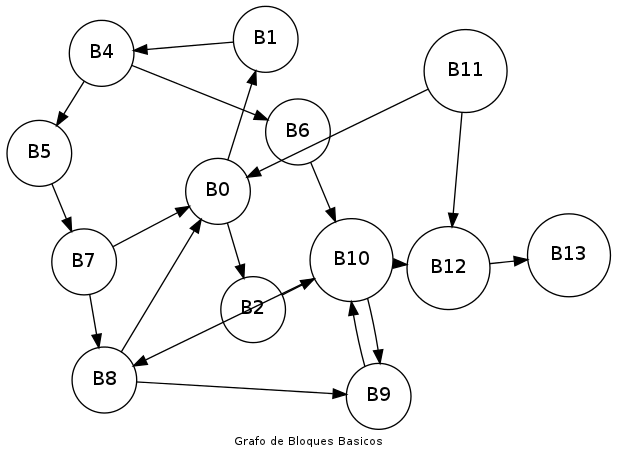
\includegraphics[width=\textwidth]{bla.png}

\end{document}
